\section{Graph Parsing Algorithm}

We propose a context-free language constrained path problem solution which allows to create finite representation of parse forest which contains trees for all satisfied paths in graph.
Finite representation of result set with structure related to specified grammar may be useful not only for results understanding and processing but also for query debugging especially for complex queries. 

Our solution is based on generalized LL (GLL)~\cite{scott2010gll, FastPracticalGLL} parsing algorithm which allows to process arbitrary (including left-recursive and ambiguous) context-free grammars with worst-case cubic time complexity and linear for LL grammars. 

\subsection{Generalized LL Parsing Algorithm}

In classical LL algorithm we have pointer in input and pointer in grammar of form $n \rightarrow \alpha \cdot \beta $ --- grammar slot. 

\begin{enumerate}
\item 
\item
\item
\item
\end{enumerate}

In case (2) we can use $FIRST$ set to choose single variant. 
But sometimes it is not possible to select only one path to continue parsing and it does not allow to use LL parsing algorithm.
Generalized LL algorithm handle all possible paths in this case. 
Instead of immediate processing of all variants GLL uses descriptors mechanism to store all possible branches and process them sequentially. 
Descriptor is a quadriple $(L, s, j, a)$ where $L$ is a grammar slot, $s$ is a stack node, $j$ is a position in the input, and $a$ is a node of derivation tree. 

Stack in parsing process is used to store return information for the parser --- a name of function which would be called when current function will finish computing. 
As previously mentioned, generalized parsers process all possible derivation branches and for every branch parser must store it's own stack. It leads to infinite stack grow.  
Tomita-style graph structured stack (GSS)~\cite{Tomita} allows to combine stacks to solve this problem.
In GLL each GSS node contains a pair of position in input and grammar slot. 

Detailed description of GLL parsing algorithm is available in this article~\cite{GLL}. Pseudocode of stack and tree manipulation functions can be found in Appendix~\ref{GLLCode}.

$R$ ---   
We use table version~\cite{TableGLL} instead of code generation.

\begin{algorithm}[h]
\begin{algorithmic}[1]
\caption{Control functions}
\label{mainFunctions}
\Function{dispatcher}{}
  \If{$R.Count \neq 0$}  
      \State{$(L,v,i,cN) \gets R.Get()$}
      \State{$cR \gets dummy$}
      \State{$dispatch \gets false$}
  \Else
      \State{$stop \gets true$}
  \EndIf
\EndFunction

\Function{processing}{}
  \State{$dispatch \gets true$}
  \Switch{$L$}
  \Case{$(X \rightarrow \alpha \cdot x \beta)$ where $x = input[i + 1])$}
       \If{$cN = dummyAST$} 
          \State{$cN \gets \Call{getNodeT}{i}$} 
       \Else 
          \State{$cR \gets \Call{getNodeT}{i}$}
       \EndIf
       \State{$i \gets i + 1$}
       \State{$L \gets (X \rightarrow \alpha x \cdot \beta)$}
       \If{$cR \neq dummy$}
          \State{$cN \gets \Call{getNodeP}{L, cN, cR}$} 
       \EndIf
       \State{$dispatch \gets false$}        
  \EndCase
  \Case{$(X \rightarrow \alpha \cdot x \beta)$ where $x$ is nonterminal}
       \State{$v \gets$ \Call{create}{$(X \rightarrow \alpha x \cdot \beta), v, i, cN$}}
       \State{$slots \gets pTable[x][input[i]]$}
       \ForAll{$L \in slots$}
          \State{\Call{add}{L,v,i,dummy}} 
       \EndFor
  \EndCase
  \Case{$(X \rightarrow \alpha \cdot )$}
       \State{\Call{pop}{v,i,cN}} 
  \EndCase
  \Case{$(S \rightarrow \alpha \cdot )$ when $S$ is start nonterminal}
       \State{final result processing and error notification} 
  \EndCase
  \EndSwitch
\EndFunction

\Function{control}{}
  \While{not $stop$}  
      \If{$dispatch$}
        \State{\Call{dispatcher}{}}
      \Else
         \State{\Call{processing}{}}
      \EndIf
  \EndWhile
\EndFunction

\end{algorithmic}
\end{algorithm}

There are more than one tree for ambiguous grammar and generalized algorithms builds all derivation trees. Special data structure --- SPPF --- is used to reduce space required for tree storage.


\subsection{Shared packed parse forest}

Shared Packed Parse Forest (SPPF)~\cite{SPPF} is a special data structure for derivation forest compact representation which allow to reuse common nodes and subtrees.
As a result multiple derivation trees, which can be produced in case of ambiguous grammar, can be compressed in one SPPF with optimal reusing of common parts.  
Binarized form of SPPF proposed in~\cite{brnglr} and it allow to achieve worst-case cubic space complexity.
GLL can use SPPF~\cite{gllParsingTree} for results representation achieve cubic space complexity with binarised version.

Let we present an example of SPPF for ambiguous grammar $G_0$ (pic~\ref{grammarG0}).

\begin{figure}[h]
   \begin{center}
\begin{verbatim}
   0: s = eps
   1: s = A s B
   2: s = s s
\end{verbatim}
   \caption{Grammar $G_0$}
   \label{grammarG0}        
   \end{center}
\end{figure}


Let we parse the sentence \verb|"ABABAB"|. 
There are two different leftmost derivations of this sentence in grammar $G_0$, hence SPPF should contains two different trees and it is presented in figure~\ref{sppfSample}: result SPPF(fig. ~\ref{sppf}) and trees for derivation 1(fig.~\ref{tree1}) and derivation 2(fig.~\ref{tree2}) respectively. 
 
\begin{figure*}[ht]
    \begin{center}
    \centering
    \begin{subfigure}[b]{0.3\textwidth}
        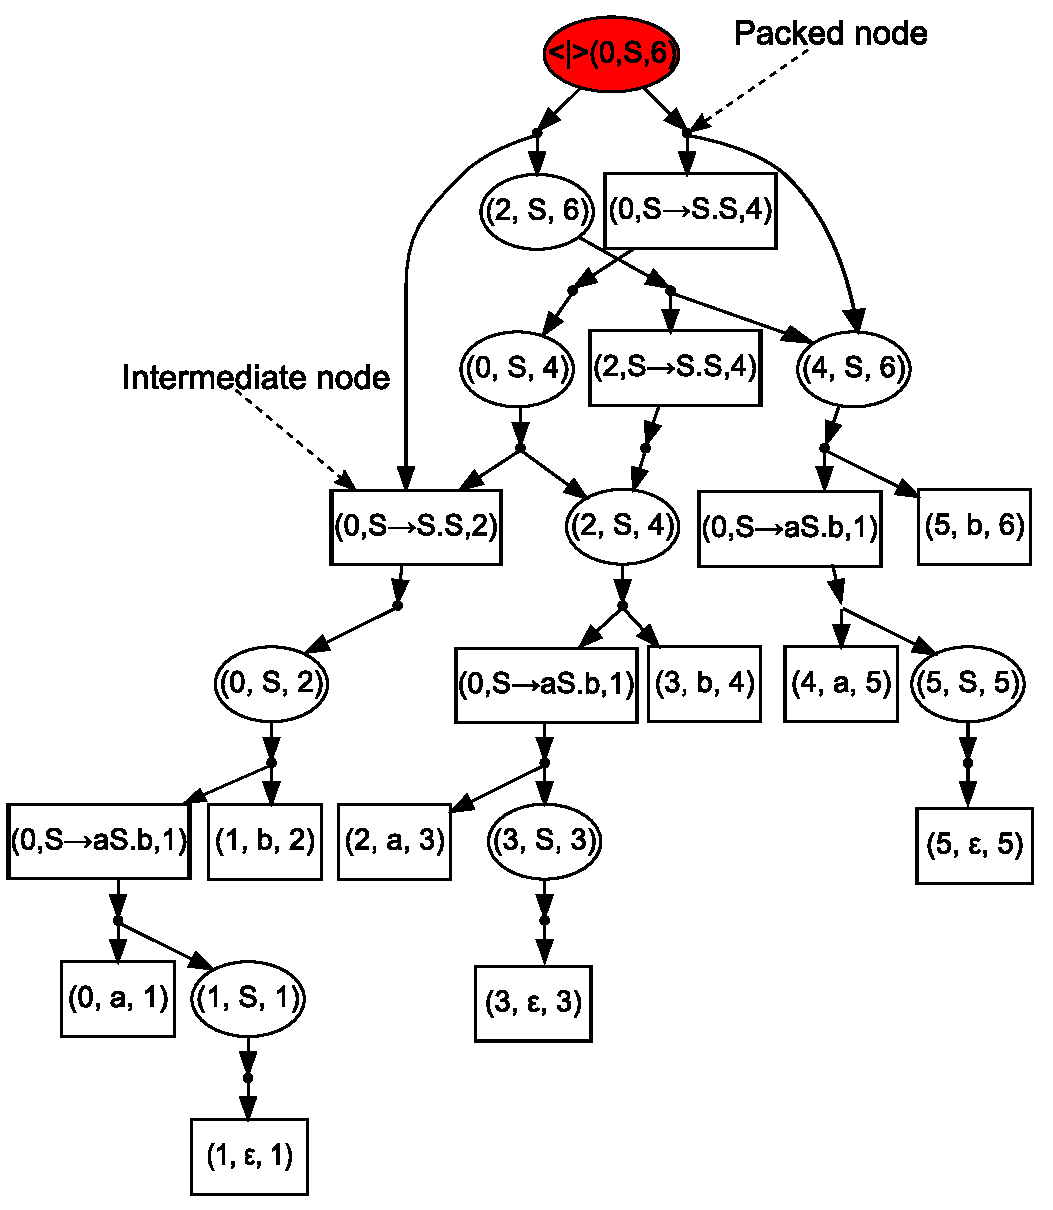
\includegraphics[width=\textwidth]{dot/Brackets.pdf}
        \caption{SPPF}
        \label{sppf}        
    \end{subfigure}
    ~
    \begin{subfigure}[b]{0.3\textwidth}
        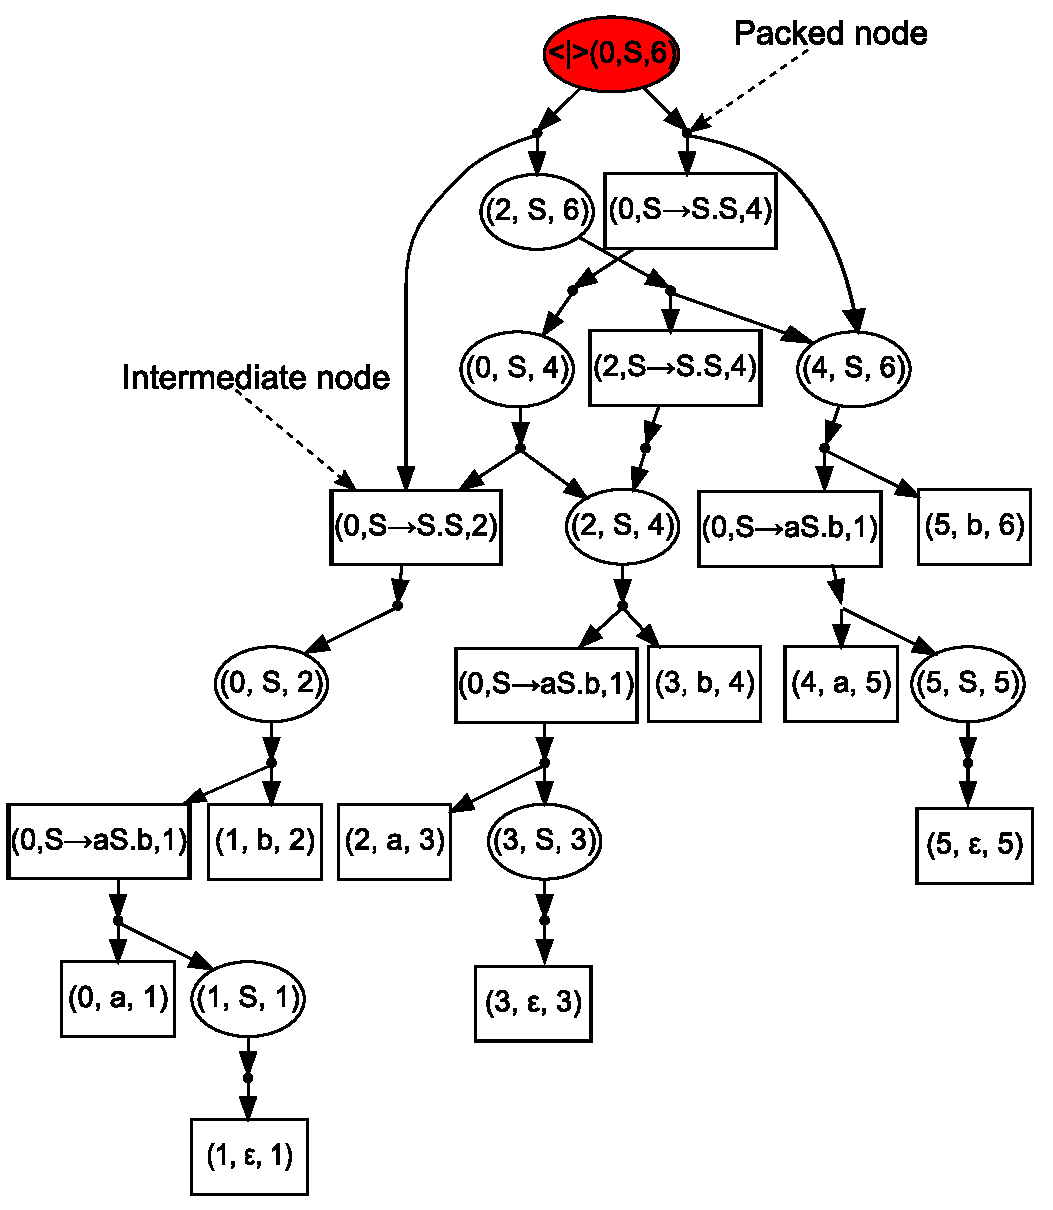
\includegraphics[width=\textwidth]{dot/Brackets.pdf}
        \caption{Tree for derivation 1}
        \label{tree1}        
    \end{subfigure}
    ~
    \begin{subfigure}[b]{0.3\textwidth}
        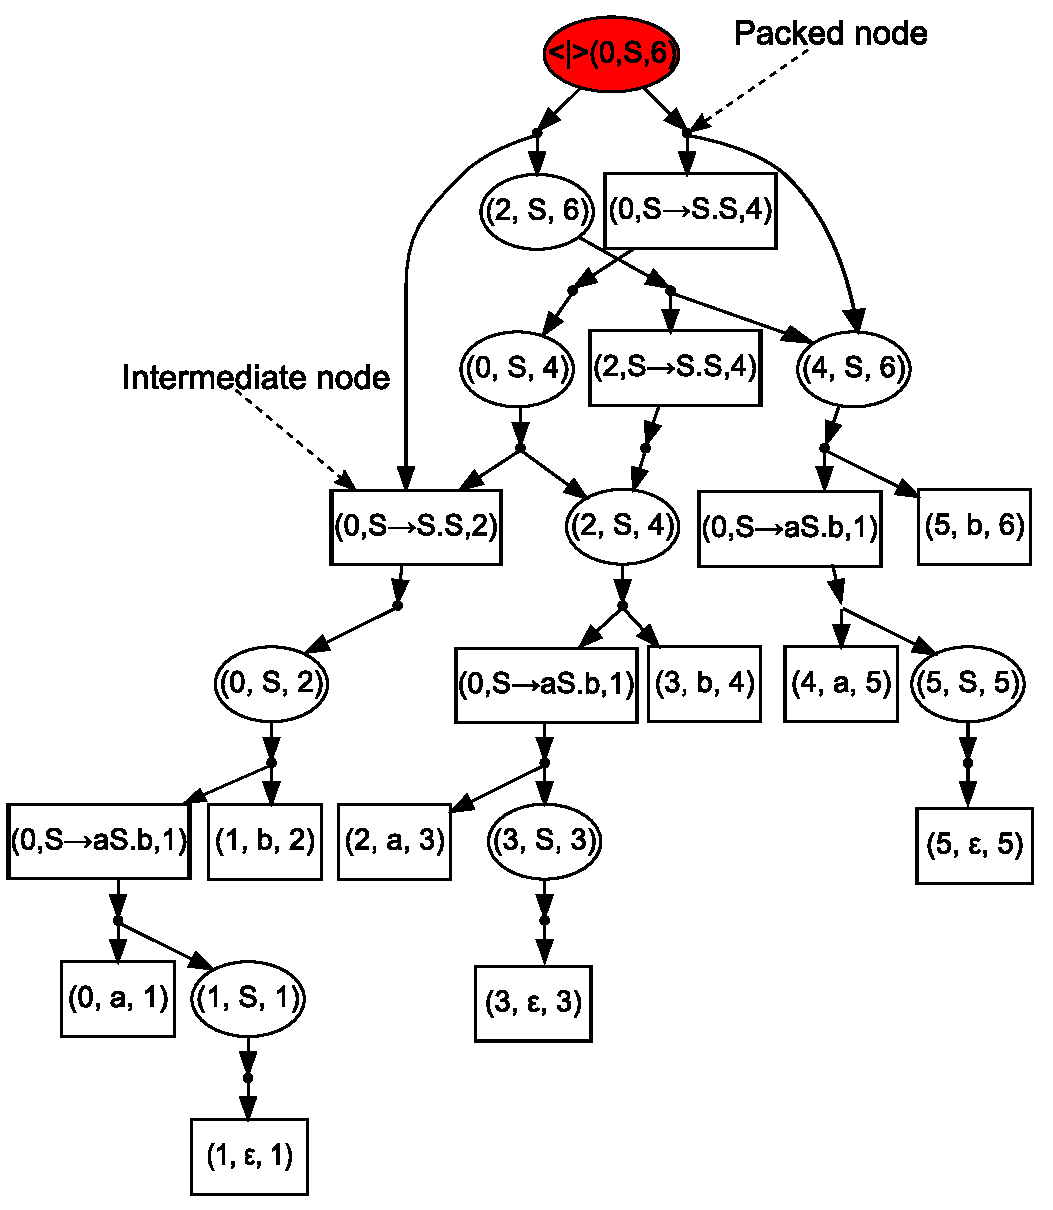
\includegraphics[width=\textwidth]{dot/Brackets.pdf}
        \caption{Tree for derivation 2}
        \label{tree2}        
    \end{subfigure}
    \caption{SPPF for sentence \textbf{\texttt{"(1)(2)(3)"}} and grammar $G_0$}
    \label{sppfSample}
    \end{center}                
\end{figure*}

Binarised SPPF can be represented as a graph where each node has one of four types which described below with corresponded graphical notation.

\begin{itemize}
    \item Node with rectangle shape labeled with $(i, T, j)$ is terminal node.     
    \item Node with oval shape labeled with $(i, N, j)$ is nonterminal node. 
    This node denote that there is at least one derivation for substring $\alpha$ from position $i$ to position $j$ in input string $\omega$ such that $N \Rightarrow^*_G \alpha, \alpha = \omega[i..j-1] $.
    All derivation trees for given substring and nonterminal can be extracted from SPPF by left-to-right top-down graph traversal started from respective node. 
    We use filled nonterminal node labeled with $(<\mkern-11mu | \mkern-11mu> (i, N, j))$ for denote that there are more then one derivations from nonterminal $N$ for substring from $i$ to $j$.
    \item Intermediate node with label $(i,t,j)$ where $t$ is a grammar slot. We use dot shape for these nodes and omit label because it is important only for SPPF constriction.
	Subgraph with root in such node is one variant of derivation in case when parent is nonterminal node with label $(<\mkern-9mu | \mkern-9mu> (i, N, j))$.
    \item Node with rectangle shape and label $(N : \gamma \cdot, k)$ is a packed node.
\end{itemize}
One of nonterminal nodes can be marked as 'root' --- node for start nonterminal. Tuple of positions $(i,j)$ which represent start and end of substring is \textit{extension} of node.

Further in our examples we will remove redundant intermediate and packed nodes from SPPF to simplify it and decrease size of structure.

\subsection{GLL-based graph parsing}

In this section we present such modification of GLL algorithm, that for input graph $M$, set of start vertices $V_s\subseteq V$, set of final vertices $V_f\subseteq V$, grammar $G_1$, it return SPPF which contains all derivation trees for all paths $p$ in $M$, such that $\Omega(p) \in L(G_1)$, and $p.start \in V_s, p.end \in V_f$.

First of all note that input string for classical parser is a linear graph, and positions in input is vertices of this graph.
This observation can be generalized to arbitrary graph with remark that in the position we have not only one next symbol, but set of labels of all outgoing edges for given vertex. 
Thus in order to use GLL for graph parsing we need to use graph vertices as position in input and modify \textbf{Processing} function to allow to process more then one "next symbol".
Required modifications presented in listing~\ref{modifAlgo}.
Small modification also required for initialization of $R$ set: it is necessary to add not only one initial descriptor but set of descriptors for all vertices in $V_s$.
All other functions can be reused from original algorithm without any changes.

\begin{algorithm}[h]
\begin{algorithmic}[1]
\caption{\textbf{Processing} function modified in order to process arbitrary directed graph}
\label{modifAlgo}
\Function{processing}{}
  \State{$dispatch \gets true$}
  \Switch{$L$}
  \Case{$(X \rightarrow \alpha \cdot x \beta)$ where $x$ is terminal}
	   \ForAll{$\{ e | e \in input.outEdges(i), tag(e) = x \}$}
	   \State{$new\_cN \gets cN$}
       \If{$new\_cN = dummyAST$} 
          \State{$new\_cN \gets \Call{getNodeT}{e}$} 
       \Else 
          \State{$new\_cR \gets \Call{getNodeT}{e}$}
       \EndIf
       \State{$L \gets (X \rightarrow \alpha x \cdot \beta)$}
       \If{$new\_cR \neq dummy$}
          \State{$new\_cN \gets \Call{getNodeP}{L, new\_cN, new\_cR}$} 
       \EndIf
	   \State{\Call{add}{L,v,target(e),new\_cN}}
	   \EndFor
  \EndCase
  \Case{$(X \rightarrow \alpha \cdot x \beta)$ where $x$ is nonterminal}
       \State{$v \gets$ \Call{create}{$(X \rightarrow \alpha x \cdot \beta), v, i, cN$}}
       \State{$slots \gets \bigcup_{e \in input.OutEdges(i)} pTable[x][e.Token]$}
       \ForAll{$L \in slots$}
          \State{\Call{add}{L,v,i,dummy}} 
       \EndFor
  \EndCase
  \Case{$(X \rightarrow \alpha \cdot )$}
       \State{\Call{pop}{v,i,cN}} 
  \EndCase
  \Case{$\_$}
       \State{final result processing and error notification} 
  \EndCase
  \EndSwitch
\EndFunction

\end{algorithmic}
\end{algorithm}





As far as we can specify sets of start and final vertices, our solution can find all paths in graph, all paths from specified vertex, all paths between specified vertices. 
Also SPPF represents a structure of paths in terms of derivation which allow to get more useful information about result. 

A bit more on correctness.!!!!!
